\documentclass[11pt]{article}
\usepackage[textwidth=18.0cm, textheight=23.0cm, top=2.0cm]{geometry}
\usepackage{pst-all}
\usepackage{amssymb}
\usepackage{tikz}
\usepackage{underscore}\begin{document}
\pagestyle{empty}


ClassName: \underline{\textbf{Class_10.2bp-19}}
\par
BinSize: \underline{\textbf{100 × 100}}
\par
ReduceSize: \underline{\textbf{100 × 100}}
\par
TypeNum: \underline{\textbf{40}}
\par
Num: \underline{\textbf{40}}
\par
OutS: \underline{\textbf{90000}}
\par
InS: \underline{\textbf{71636}}
\par
Rate: \underline{\textbf{0.796}}
\par
UB: \underline{\textbf{9}}
\par
LB0: \underline{\textbf{9}}
\par
LB: \underline{\textbf{9}}
\par
LBWithCut: \underline{\textbf{9}}
\par
NodeCut: \underline{\textbf{0}}
\par
ExtendedNodeCnt: \underline{\textbf{1}}
\par
GenNodeCnt: \underline{\textbf{1}}
\par
PrimalNode: \underline{\textbf{0}}
\par
ColumnCount: \underline{\textbf{9}}
\par
TotalCutCount: \underline{\textbf{0}}
\par
RootCutCount: \underline{\textbf{0}}
\par
LPSolverCnt: \underline{\textbf{1}}
\par
PricingSolverCnt: \underline{\textbf{0}}
\par
BranchAndBoundNum: \underline{\textbf{1}}
\par
isOpt: \underline{\textbf{true}}
\par
TimeOnPrimal: \underline{\textbf{0.000 s}}
\par
TimeOnPricing: \underline{\textbf{0.000 s}}
\par
TimeOnRmp: \underline{\textbf{0.063 s}}
\par
TotalTime: \underline{\textbf{0.110 s}}
\par
\newpage


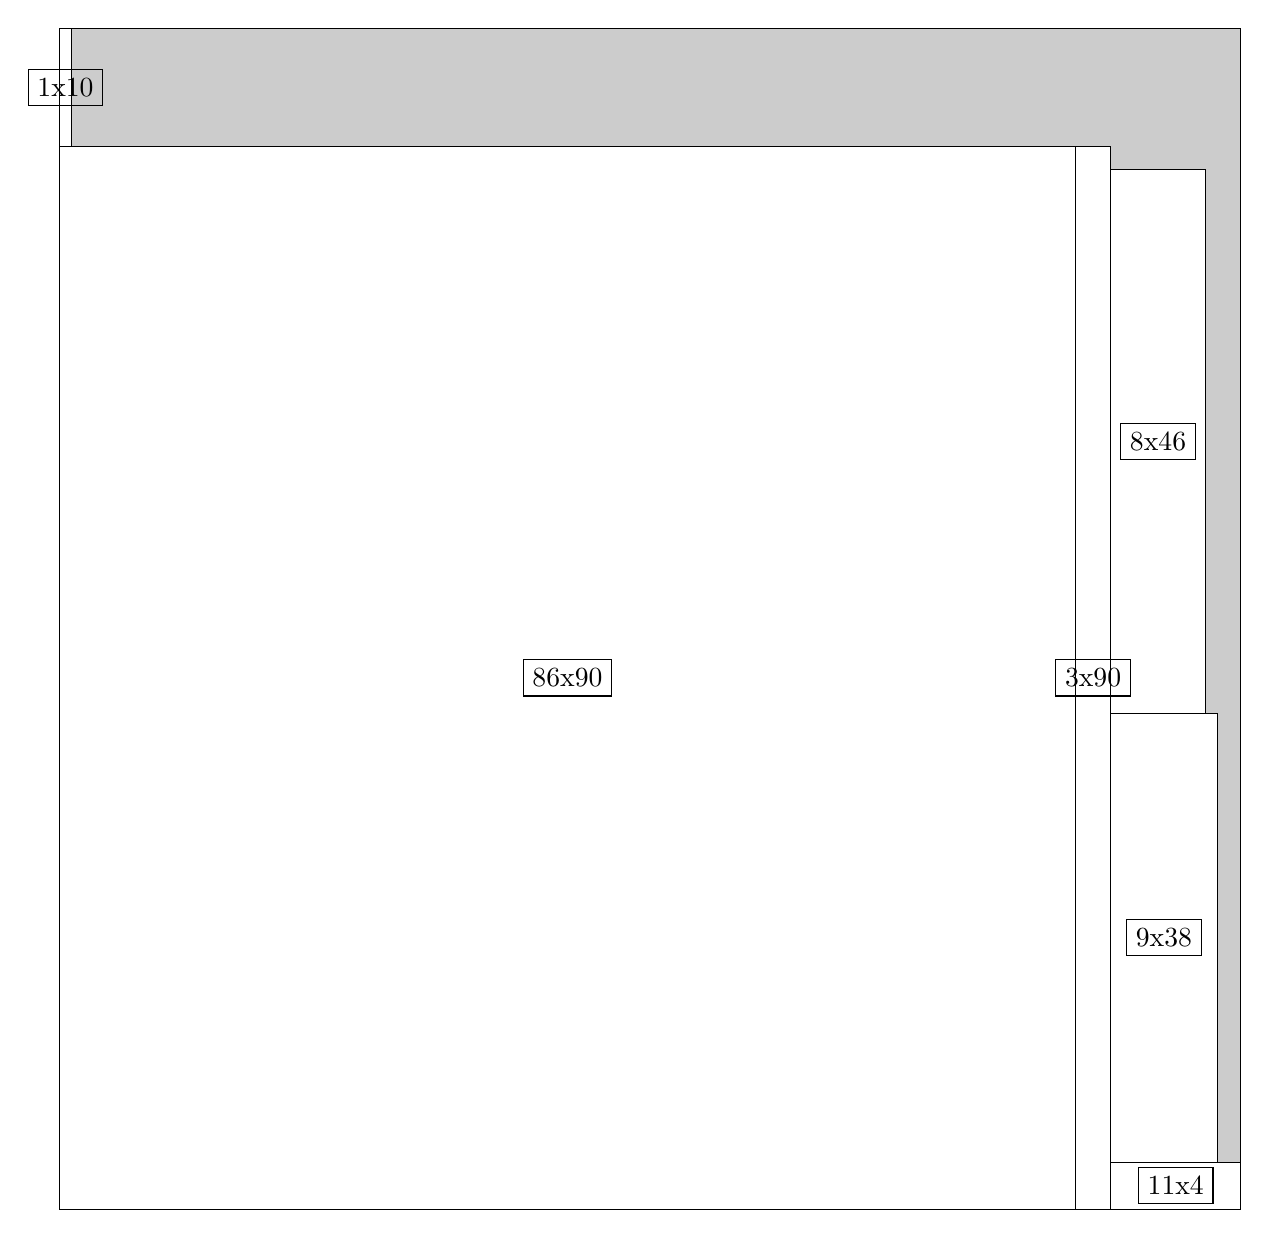
\begin{tikzpicture}[shorten >=1pt,scale=1.0,every node/.style={scale=1.0},->]
\tikzstyle{vertex}=[circle,fill=black!25,minimum size=14pt,inner sep=0pt]
\filldraw[fill=gray!40!white, draw=black] (0,0) rectangle (15.0,15.0);
\foreach \name/\x/\y/\w/\h in {86x90/0.0/0.0/12.9/13.5,8x46/13.35/6.3/1.2/6.8999999999999995,9x38/13.35/0.6/1.3499999999999999/5.7,3x90/12.9/0.0/0.44999999999999996/13.5,11x4/13.35/0.0/1.65/0.6,1x10/0.0/13.5/0.15/1.5}
\filldraw[fill=white!40!white, draw=black] (\x,\y) rectangle node[draw] (\name) {\name} ++(\w,\h);
\end{tikzpicture}


w =86 , h =90 , x =0 , y =0 , v =7740
\par
w =8 , h =46 , x =89 , y =42 , v =368
\par
w =9 , h =38 , x =89 , y =4 , v =342
\par
w =3 , h =90 , x =86 , y =0 , v =270
\par
w =11 , h =4 , x =89 , y =0 , v =44
\par
w =1 , h =10 , x =0 , y =90 , v =10
\par
\newpage


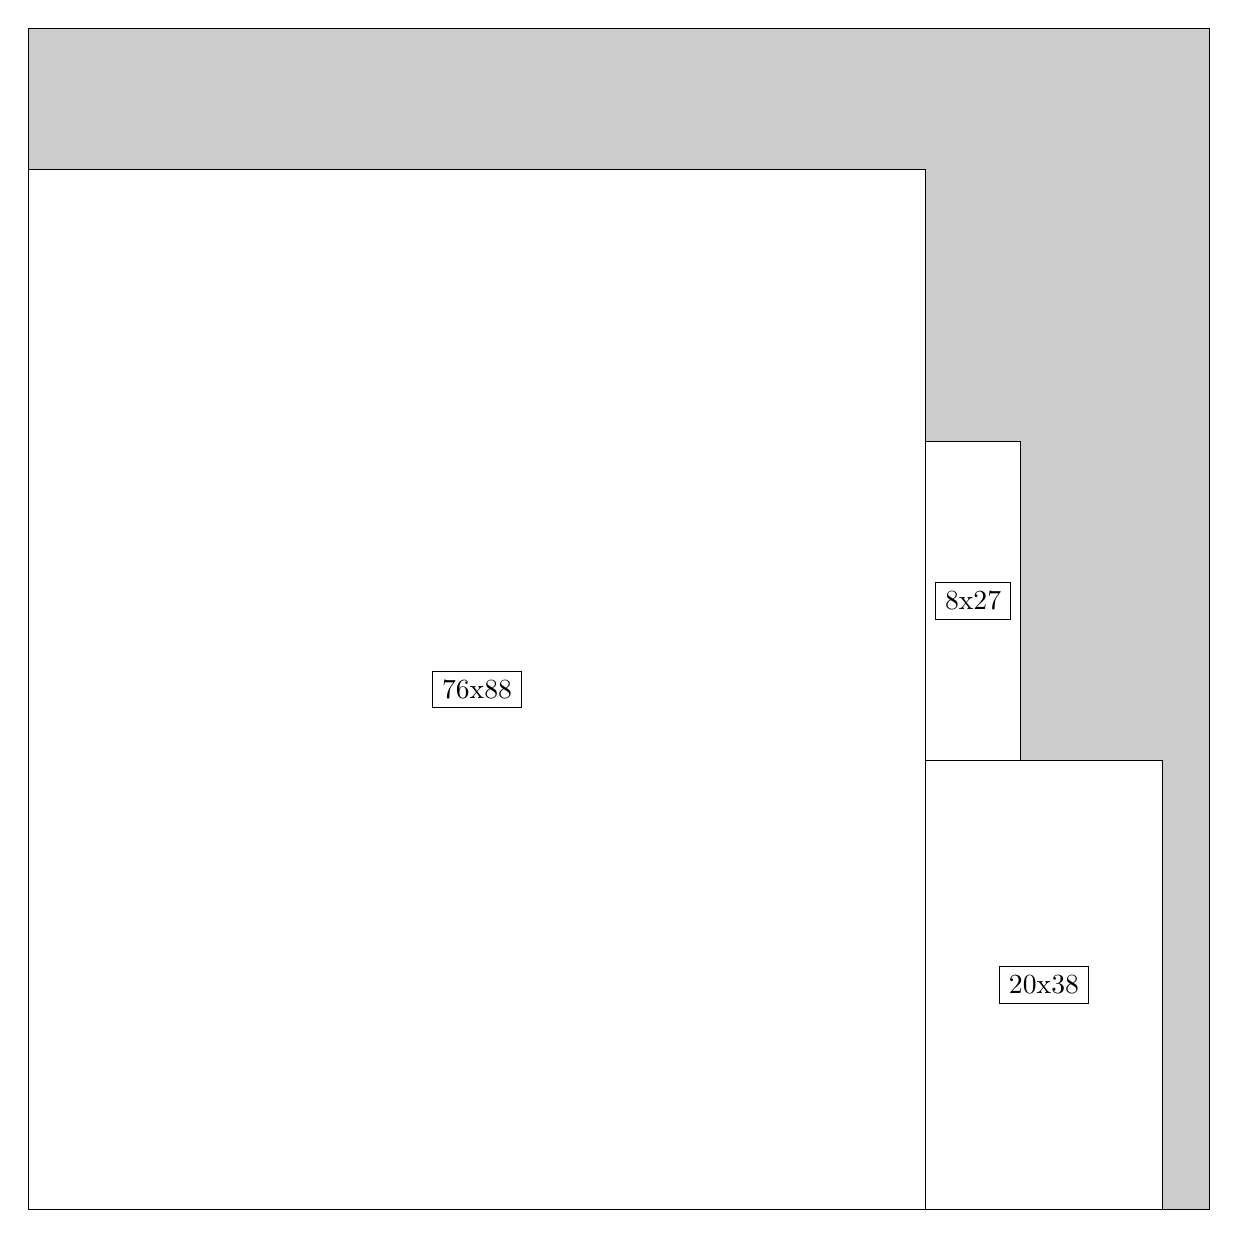
\begin{tikzpicture}[shorten >=1pt,scale=1.0,every node/.style={scale=1.0},->]
\tikzstyle{vertex}=[circle,fill=black!25,minimum size=14pt,inner sep=0pt]
\filldraw[fill=gray!40!white, draw=black] (0,0) rectangle (15.0,15.0);
\foreach \name/\x/\y/\w/\h in {76x88/0.0/0.0/11.4/13.2,20x38/11.4/0.0/3.0/5.7,8x27/11.4/5.7/1.2/4.05}
\filldraw[fill=white!40!white, draw=black] (\x,\y) rectangle node[draw] (\name) {\name} ++(\w,\h);
\end{tikzpicture}


w =76 , h =88 , x =0 , y =0 , v =6688
\par
w =20 , h =38 , x =76 , y =0 , v =760
\par
w =8 , h =27 , x =76 , y =38 , v =216
\par
\newpage


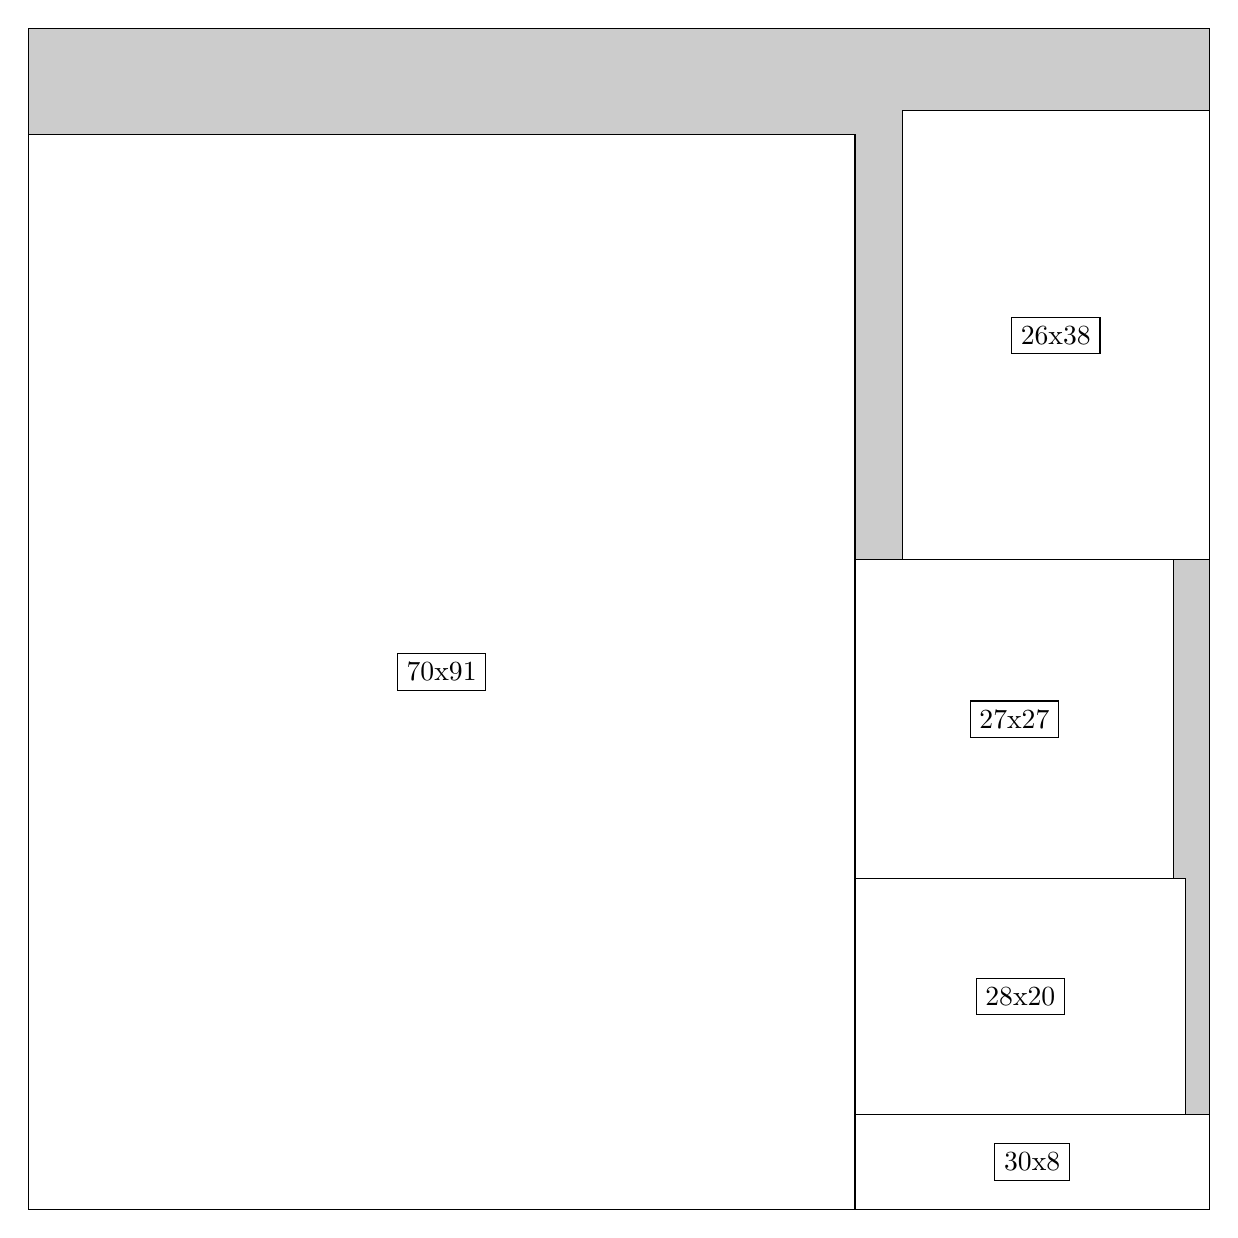
\begin{tikzpicture}[shorten >=1pt,scale=1.0,every node/.style={scale=1.0},->]
\tikzstyle{vertex}=[circle,fill=black!25,minimum size=14pt,inner sep=0pt]
\filldraw[fill=gray!40!white, draw=black] (0,0) rectangle (15.0,15.0);
\foreach \name/\x/\y/\w/\h in {70x91/0.0/0.0/10.5/13.65,26x38/11.1/8.25/3.9/5.7,27x27/10.5/4.2/4.05/4.05,30x8/10.5/0.0/4.5/1.2,28x20/10.5/1.2/4.2/3.0}
\filldraw[fill=white!40!white, draw=black] (\x,\y) rectangle node[draw] (\name) {\name} ++(\w,\h);
\end{tikzpicture}


w =70 , h =91 , x =0 , y =0 , v =6370
\par
w =26 , h =38 , x =74 , y =55 , v =988
\par
w =27 , h =27 , x =70 , y =28 , v =729
\par
w =30 , h =8 , x =70 , y =0 , v =240
\par
w =28 , h =20 , x =70 , y =8 , v =560
\par
\newpage


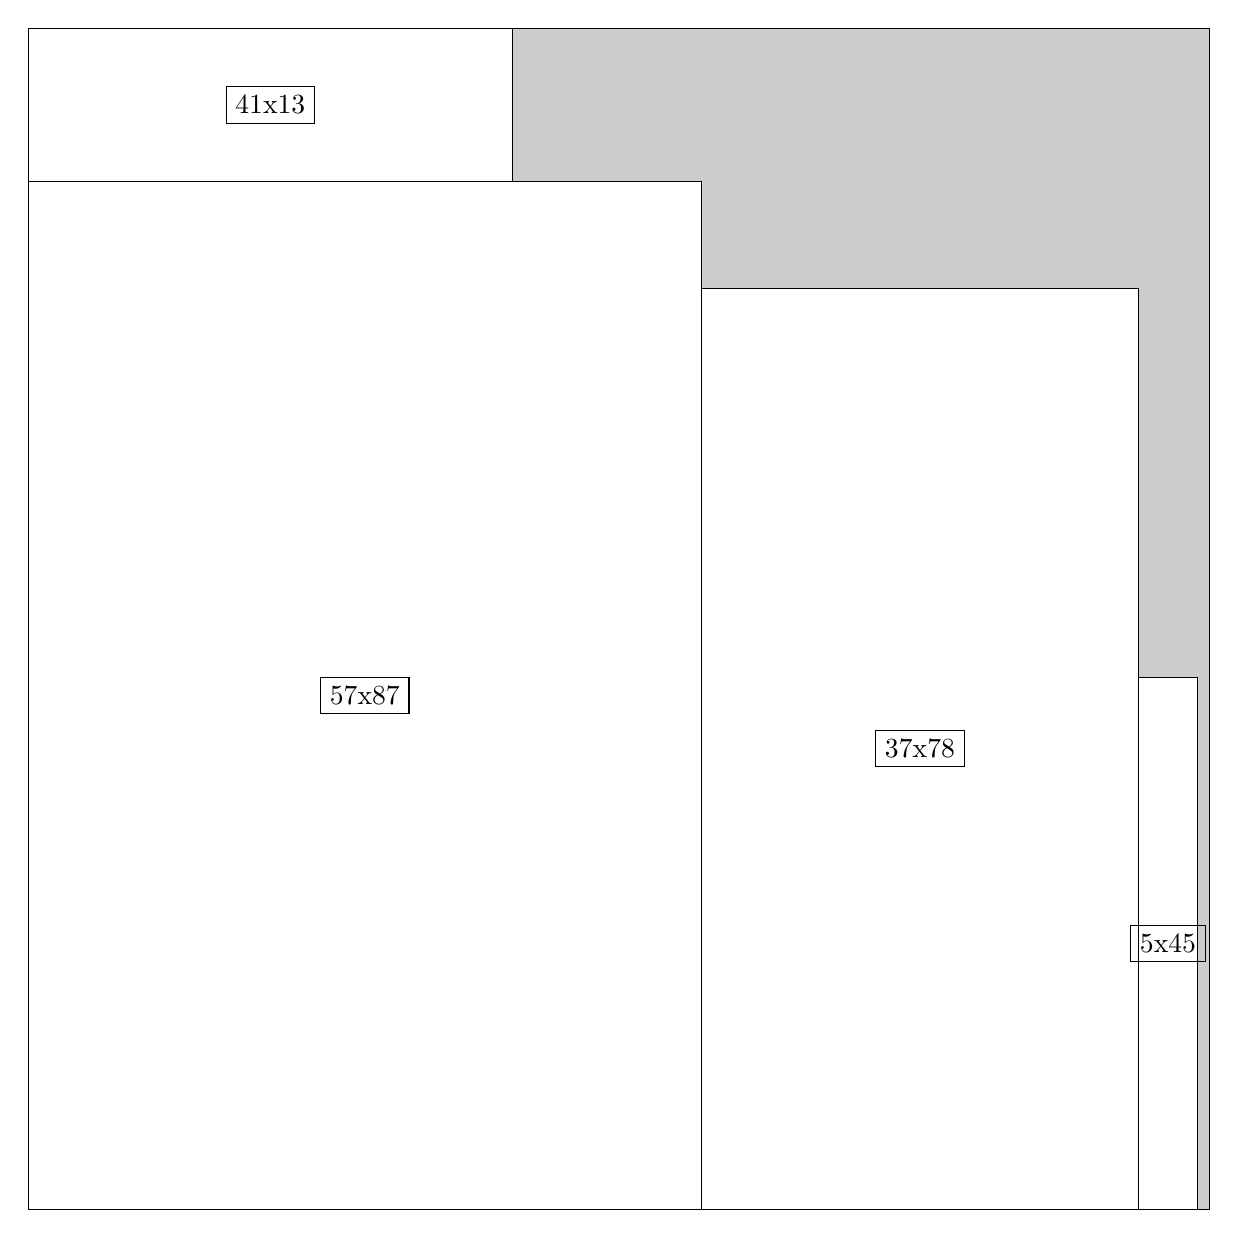
\begin{tikzpicture}[shorten >=1pt,scale=1.0,every node/.style={scale=1.0},->]
\tikzstyle{vertex}=[circle,fill=black!25,minimum size=14pt,inner sep=0pt]
\filldraw[fill=gray!40!white, draw=black] (0,0) rectangle (15.0,15.0);
\foreach \name/\x/\y/\w/\h in {57x87/0.0/0.0/8.549999999999999/13.049999999999999,37x78/8.549999999999999/0.0/5.55/11.7,41x13/0.0/13.049999999999999/6.1499999999999995/1.95,5x45/14.1/0.0/0.75/6.75}
\filldraw[fill=white!40!white, draw=black] (\x,\y) rectangle node[draw] (\name) {\name} ++(\w,\h);
\end{tikzpicture}


w =57 , h =87 , x =0 , y =0 , v =4959
\par
w =37 , h =78 , x =57 , y =0 , v =2886
\par
w =41 , h =13 , x =0 , y =87 , v =533
\par
w =5 , h =45 , x =94 , y =0 , v =225
\par
\newpage


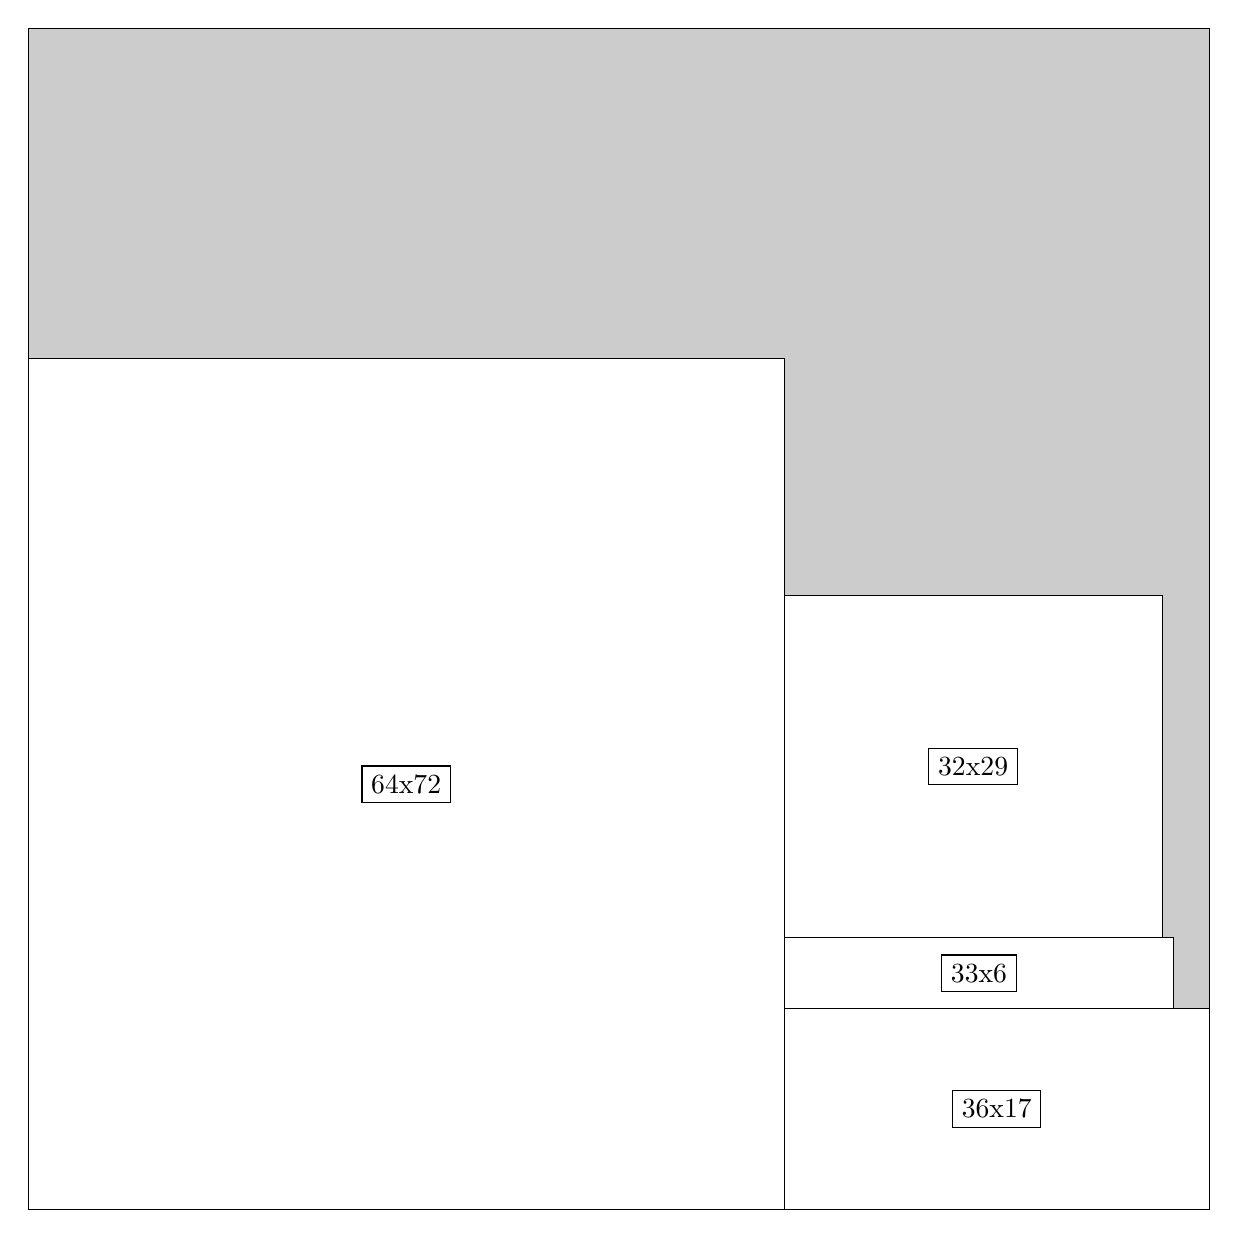
\begin{tikzpicture}[shorten >=1pt,scale=1.0,every node/.style={scale=1.0},->]
\tikzstyle{vertex}=[circle,fill=black!25,minimum size=14pt,inner sep=0pt]
\filldraw[fill=gray!40!white, draw=black] (0,0) rectangle (15.0,15.0);
\foreach \name/\x/\y/\w/\h in {64x72/0.0/0.0/9.6/10.799999999999999,32x29/9.6/3.4499999999999997/4.8/4.35,36x17/9.6/0.0/5.3999999999999995/2.55,33x6/9.6/2.55/4.95/0.8999999999999999}
\filldraw[fill=white!40!white, draw=black] (\x,\y) rectangle node[draw] (\name) {\name} ++(\w,\h);
\end{tikzpicture}


w =64 , h =72 , x =0 , y =0 , v =4608
\par
w =32 , h =29 , x =64 , y =23 , v =928
\par
w =36 , h =17 , x =64 , y =0 , v =612
\par
w =33 , h =6 , x =64 , y =17 , v =198
\par
\newpage


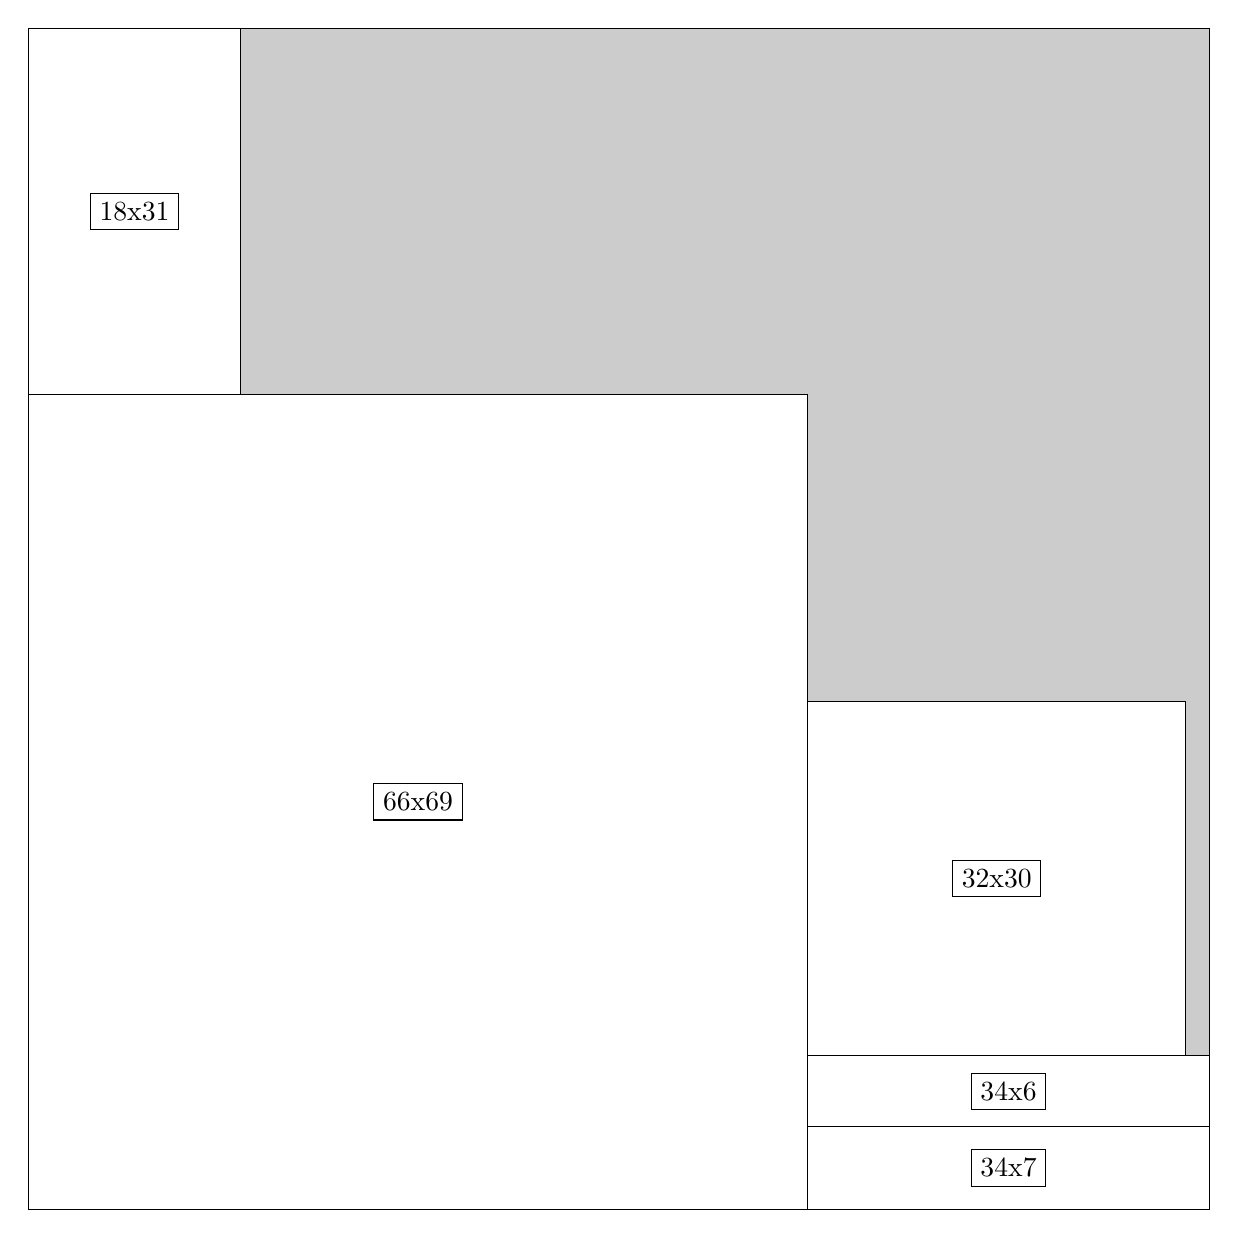
\begin{tikzpicture}[shorten >=1pt,scale=1.0,every node/.style={scale=1.0},->]
\tikzstyle{vertex}=[circle,fill=black!25,minimum size=14pt,inner sep=0pt]
\filldraw[fill=gray!40!white, draw=black] (0,0) rectangle (15.0,15.0);
\foreach \name/\x/\y/\w/\h in {66x69/0.0/0.0/9.9/10.35,32x30/9.9/1.95/4.8/4.5,18x31/0.0/10.35/2.6999999999999997/4.6499999999999995,34x7/9.9/0.0/5.1/1.05,34x6/9.9/1.05/5.1/0.8999999999999999}
\filldraw[fill=white!40!white, draw=black] (\x,\y) rectangle node[draw] (\name) {\name} ++(\w,\h);
\end{tikzpicture}


w =66 , h =69 , x =0 , y =0 , v =4554
\par
w =32 , h =30 , x =66 , y =13 , v =960
\par
w =18 , h =31 , x =0 , y =69 , v =558
\par
w =34 , h =7 , x =66 , y =0 , v =238
\par
w =34 , h =6 , x =66 , y =7 , v =204
\par
\newpage


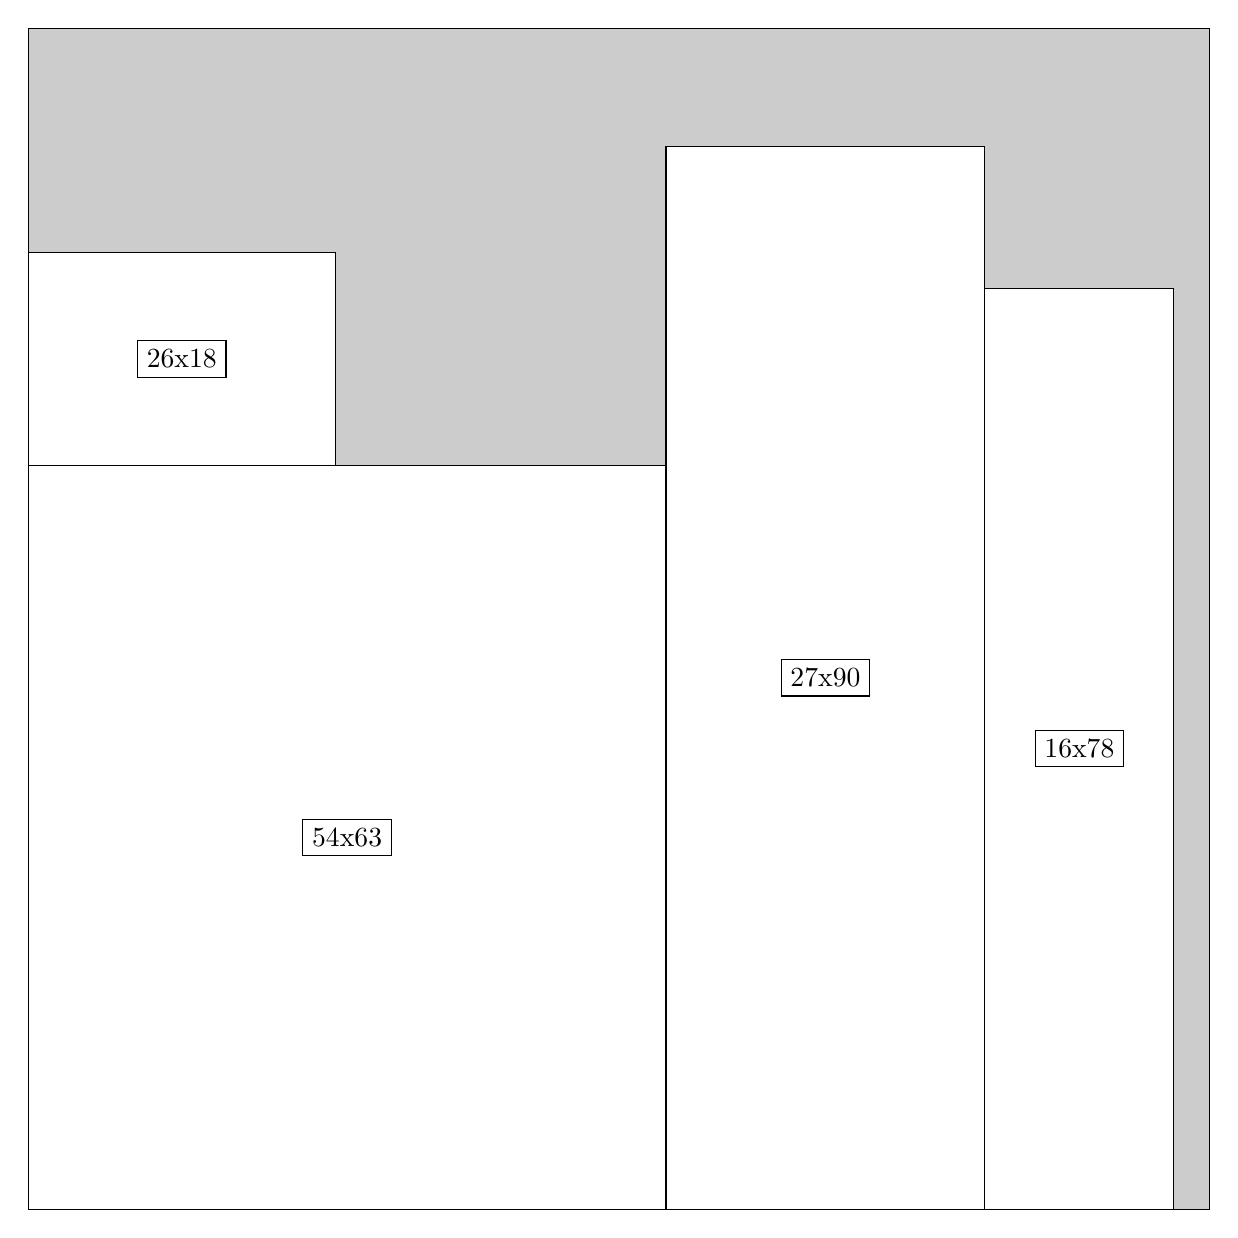
\begin{tikzpicture}[shorten >=1pt,scale=1.0,every node/.style={scale=1.0},->]
\tikzstyle{vertex}=[circle,fill=black!25,minimum size=14pt,inner sep=0pt]
\filldraw[fill=gray!40!white, draw=black] (0,0) rectangle (15.0,15.0);
\foreach \name/\x/\y/\w/\h in {54x63/0.0/0.0/8.1/9.45,27x90/8.1/0.0/4.05/13.5,16x78/12.15/0.0/2.4/11.7,26x18/0.0/9.45/3.9/2.6999999999999997}
\filldraw[fill=white!40!white, draw=black] (\x,\y) rectangle node[draw] (\name) {\name} ++(\w,\h);
\end{tikzpicture}


w =54 , h =63 , x =0 , y =0 , v =3402
\par
w =27 , h =90 , x =54 , y =0 , v =2430
\par
w =16 , h =78 , x =81 , y =0 , v =1248
\par
w =26 , h =18 , x =0 , y =63 , v =468
\par
\newpage


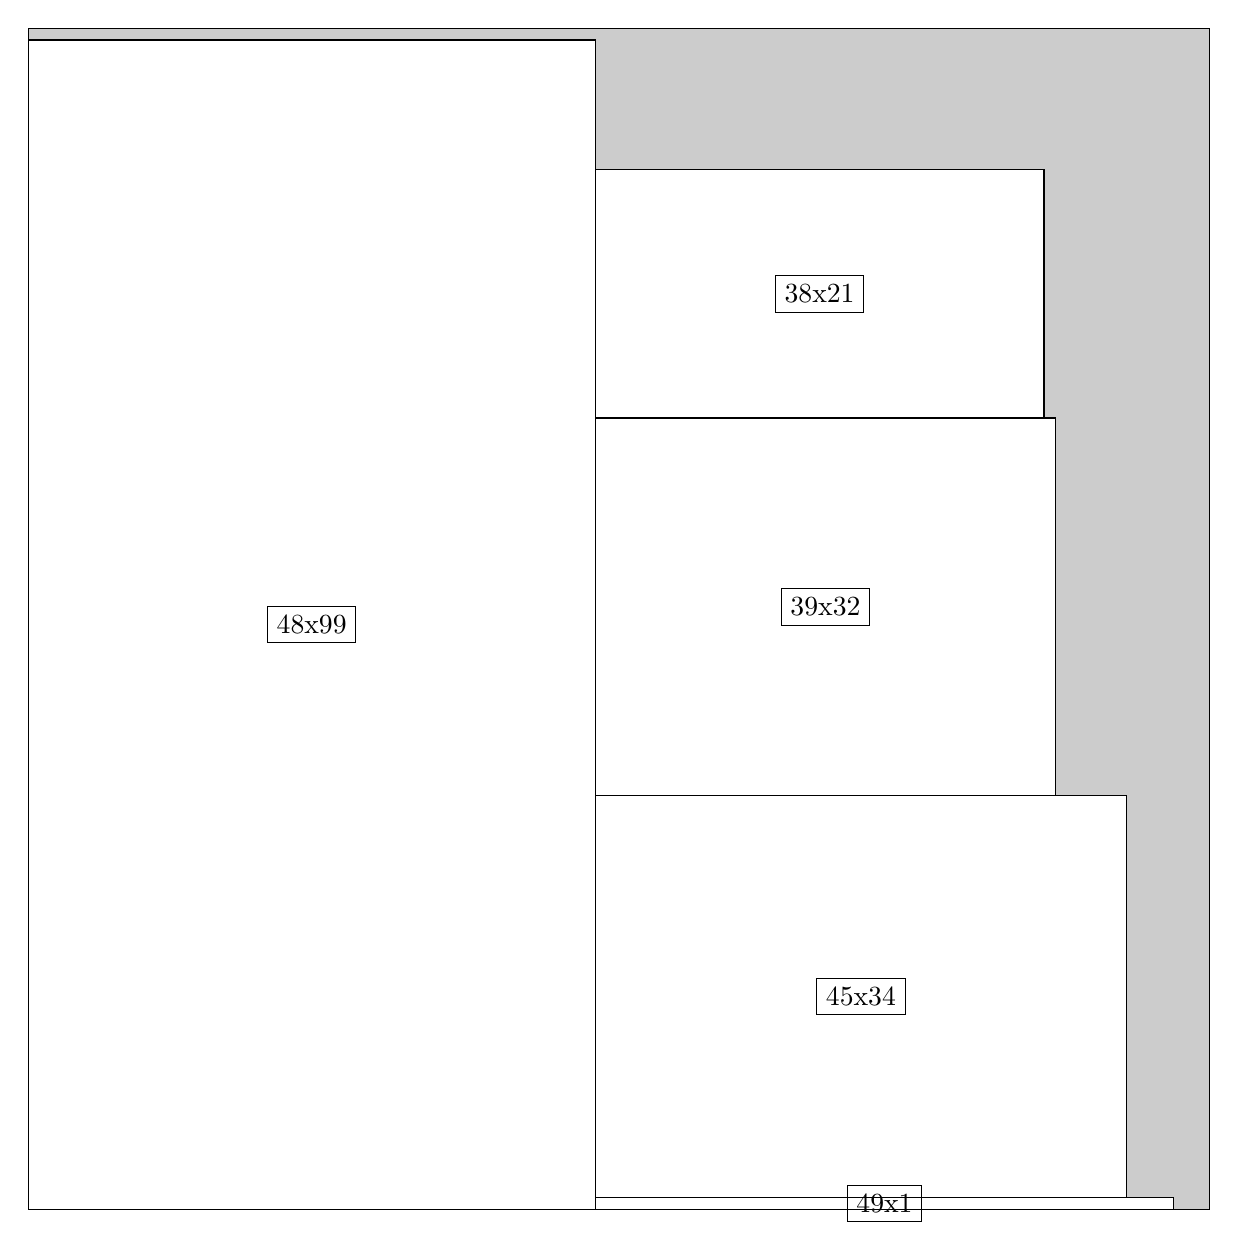
\begin{tikzpicture}[shorten >=1pt,scale=1.0,every node/.style={scale=1.0},->]
\tikzstyle{vertex}=[circle,fill=black!25,minimum size=14pt,inner sep=0pt]
\filldraw[fill=gray!40!white, draw=black] (0,0) rectangle (15.0,15.0);
\foreach \name/\x/\y/\w/\h in {48x99/0.0/0.0/7.199999999999999/14.85,45x34/7.199999999999999/0.15/6.75/5.1,39x32/7.199999999999999/5.25/5.85/4.8,38x21/7.199999999999999/10.049999999999999/5.7/3.15,49x1/7.199999999999999/0.0/7.35/0.15}
\filldraw[fill=white!40!white, draw=black] (\x,\y) rectangle node[draw] (\name) {\name} ++(\w,\h);
\end{tikzpicture}


w =48 , h =99 , x =0 , y =0 , v =4752
\par
w =45 , h =34 , x =48 , y =1 , v =1530
\par
w =39 , h =32 , x =48 , y =35 , v =1248
\par
w =38 , h =21 , x =48 , y =67 , v =798
\par
w =49 , h =1 , x =48 , y =0 , v =49
\par
\newpage


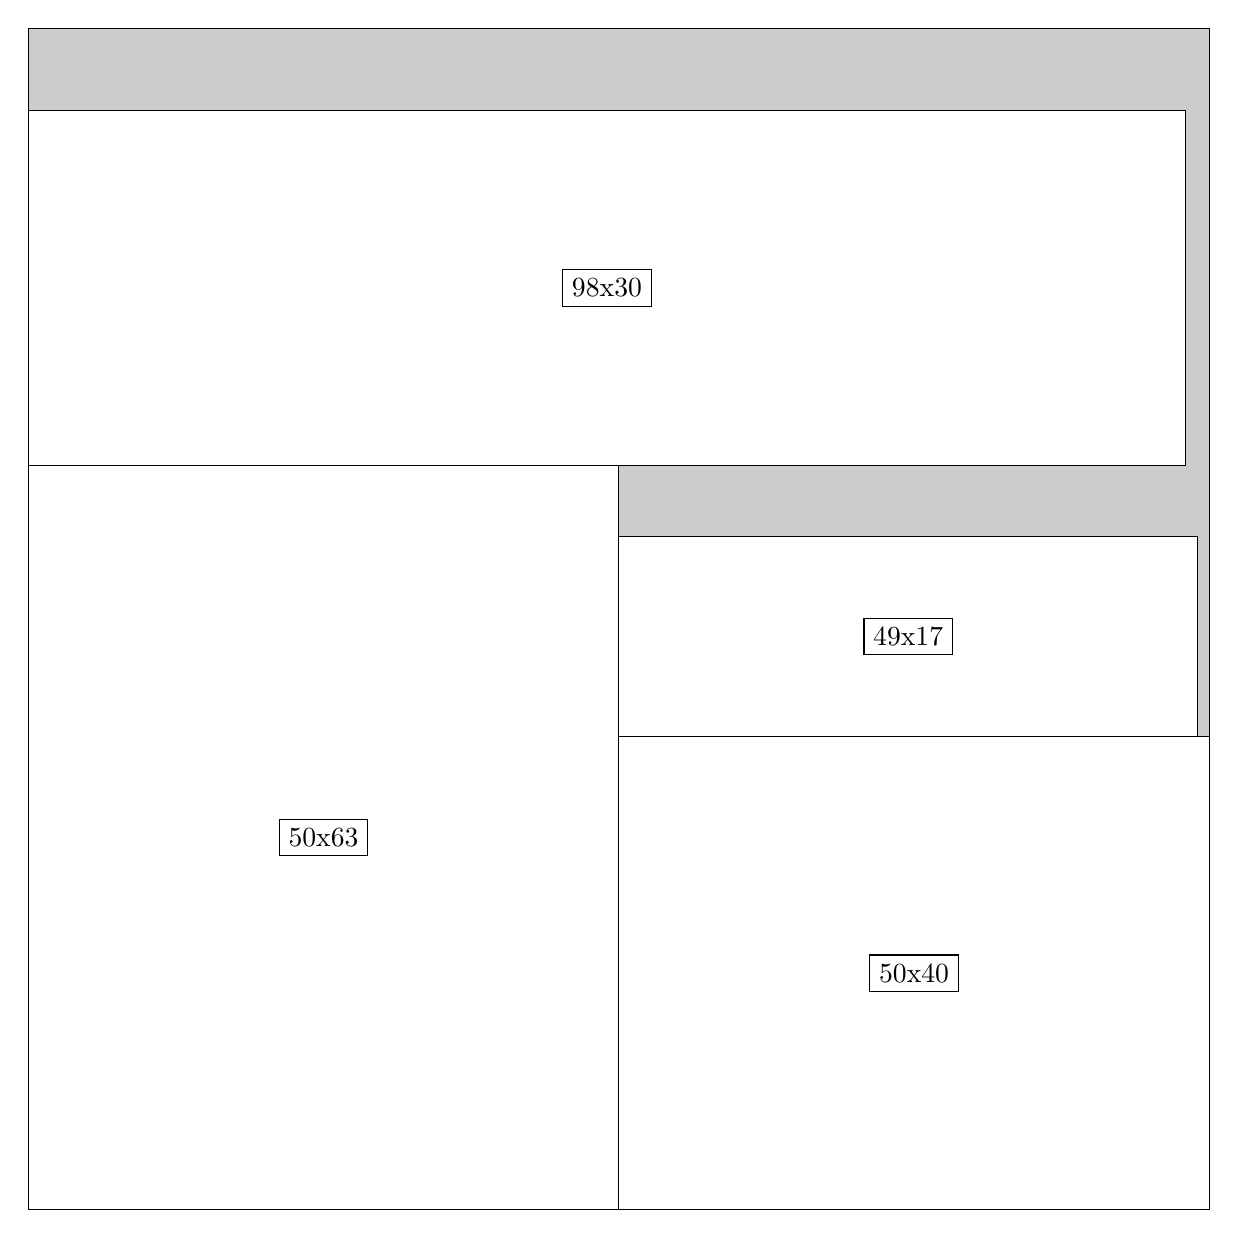
\begin{tikzpicture}[shorten >=1pt,scale=1.0,every node/.style={scale=1.0},->]
\tikzstyle{vertex}=[circle,fill=black!25,minimum size=14pt,inner sep=0pt]
\filldraw[fill=gray!40!white, draw=black] (0,0) rectangle (15.0,15.0);
\foreach \name/\x/\y/\w/\h in {50x63/0.0/0.0/7.5/9.45,98x30/0.0/9.45/14.7/4.5,50x40/7.5/0.0/7.5/6.0,49x17/7.5/6.0/7.35/2.55}
\filldraw[fill=white!40!white, draw=black] (\x,\y) rectangle node[draw] (\name) {\name} ++(\w,\h);
\end{tikzpicture}


w =50 , h =63 , x =0 , y =0 , v =3150
\par
w =98 , h =30 , x =0 , y =63 , v =2940
\par
w =50 , h =40 , x =50 , y =0 , v =2000
\par
w =49 , h =17 , x =50 , y =40 , v =833
\par
\newpage


\end{document}